\begin{figure}[tbh]
\centering

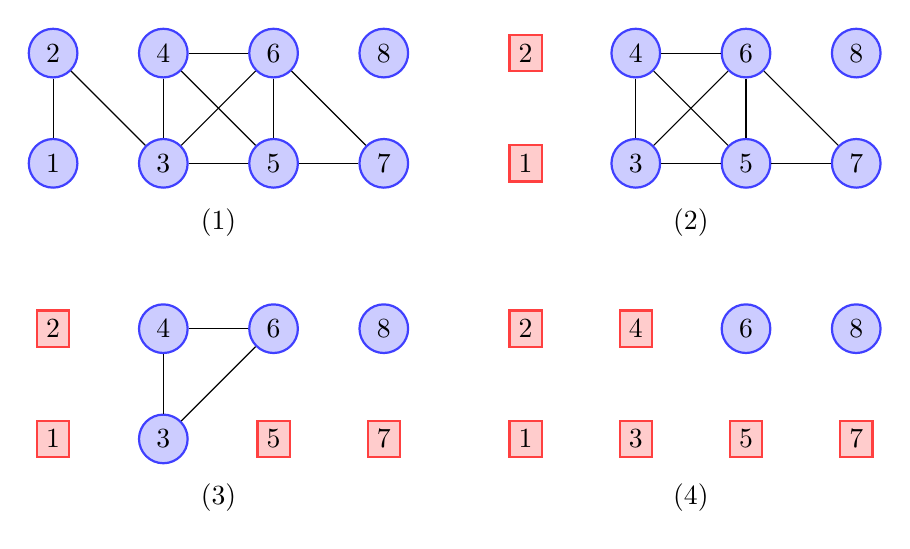
\begin{tikzpicture} [node distance=1.4cm]

\tikzstyle{unmark_vertex}=[circle,thick,draw=blue!75,fill=blue!20,minimum size=5mm]
\tikzstyle{mark_vertex}=[rectangle,thick,draw=red!75,
  			  fill=red!20,minimum size=4mm]

  \begin{scope}
  	\node [unmark_vertex] (v1) {1};
  	\node [unmark_vertex] (v2) [above of=v1] {2}
  		edge (v1);
  	\node [unmark_vertex] (v3) [right of=v1] {3}
  		edge (v2);
  	\node [unmark_vertex] (v4) [right of=v2] {4}
  		edge (v3);
  	\node [unmark_vertex] (v5) [right of=v3] {5}
  		edge (v3)
  		edge (v4);
  	\node [unmark_vertex] (v6) [right of=v4] {6}
  		edge (v3)
  		edge (v4)
  		edge (v5);
  	\node [unmark_vertex] (v7) [right of=v5] {7}
  		edge (v5)
  		edge (v6);
  	\node [unmark_vertex] (v8) [right of=v6] {8};

	\node at (2.1cm, -0.75cm) {\text{(1)}};
  \end{scope}
  
  \begin{scope}[xshift=6cm]
  	\node [mark_vertex] (v1) {1};
  	\node [mark_vertex] (v2) [above of=v1] {2};
  	\node [unmark_vertex] (v3) [right of=v1] {3};
  	\node [unmark_vertex] (v4) [right of=v2] {4}
  		edge (v3);
  	\node [unmark_vertex] (v5) [right of=v3] {5}
  		edge (v3)
  		edge (v4);
  	\node [unmark_vertex] (v6) [right of=v4] {6}
  		edge (v3)
  		edge (v4)
  		edge (v5);
  	\node [unmark_vertex] (v7) [right of=v5] {7}
  		edge (v5)
  		edge (v6);
  	\node [unmark_vertex] (v8) [right of=v6] {8};

	\node at (2.1cm, -0.75cm) {\text{(2)}};
  \end{scope}
  
  \begin{scope}[yshift=-3.5cm]
  	\node [mark_vertex] (v1) {1};
  	\node [mark_vertex] (v2) [above of=v1] {2};
  	\node [unmark_vertex] (v3) [right of=v1] {3};
  	\node [unmark_vertex] (v4) [right of=v2] {4}
  		edge (v3);
  	\node [mark_vertex] (v5) [right of=v3] {5};
  	\node [unmark_vertex] (v6) [right of=v4] {6}
  		edge (v3)
  		edge (v4);
  	\node [mark_vertex] (v7) [right of=v5] {7};
  	\node [unmark_vertex] (v8) [right of=v6] {8};

	\node at (2.1cm, -0.75cm) {\text{(3)}};
  \end{scope}
  
  \begin{scope}[yshift=-3.5cm, xshift=6cm]
  	\node [mark_vertex] (v1) {1};
  	\node [mark_vertex] (v2) [above of=v1] {2};
  	\node [mark_vertex] (v3) [right of=v1] {3};
  	\node [mark_vertex] (v4) [right of=v2] {4};
  	\node [mark_vertex] (v5) [right of=v3] {5};
  	\node [unmark_vertex] (v6) [right of=v4] {6};
  	\node [mark_vertex] (v7) [right of=v5] {7};
  	\node [unmark_vertex] (v8) [right of=v6] {8};

	\node at (2.1cm, -0.75cm) {\text{(4)}};
  \end{scope}
\end{tikzpicture}

\caption{Przykład wykonania algorytmu VERTEX-COVER-EDGES-APPROX}
\label{vertex-cover-edges-approx_example}
%\small
%zakomentarzowany tekst
\end{figure}